\documentclass[border=2pt]{standalone}

% Drawing
\usepackage{tikz}
\tikzset{>=latex}
\usetikzlibrary{angles, quotes, shapes, decorations.markings, calc}

\tikzstyle{ray} = [postaction=decorate,decoration={markings,mark=at position .52 with \arrow{>}}, red, line width=1.5]

\newcommand{\point}[4]{
\draw[fill=#4] (#1) circle (2pt) node[#3] {#2};
}

\begin{document}
	
	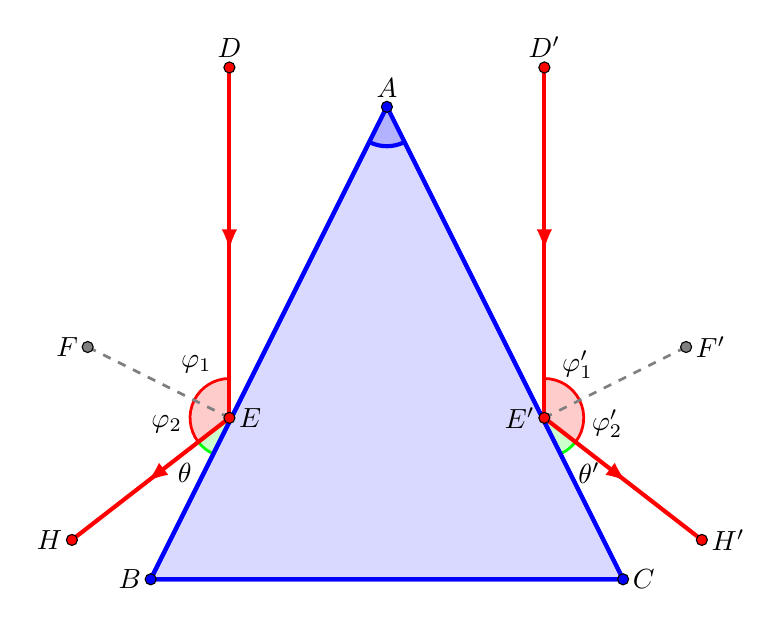
\begin{tikzpicture}
		% Axis and Grid
%		\foreach \i in {-5,...,1,...,5}
%		{
%			\node at (\i,0) {\i};
%			\node at (0,\i) {\i};
%		}
		
		% Coordinates
		\coordinate (A) at (0,6);
		\coordinate (B) at (-3,0);
		\coordinate (C) at (3,0);
		\coordinate (D) at (-2,6.5);
		\coordinate (E) at (-2,2.05);
		\coordinate (H) at (-4,0.5);
		\coordinate (D') at (2,6.5);
		\coordinate (E') at (2,2.05);
		\coordinate (H') at (4,0.5);
		\coordinate (F) at (-3.8,2.95);
		\coordinate (F') at (3.8,2.95);
		
		% Angles
		 \pic[draw=red, fill=red!20, line width=1, "$\varphi_1$", angle eccentricity=1.6] {angle = D--E--F};
		 \pic[draw=red, fill=red!20, line width=1, "$\varphi_2$", angle eccentricity=1.6] {angle = F--E--H};
		 \pic[draw=green, fill=green!20, line width=1, "$\theta$", angle eccentricity=1.8] {angle = H--E--B};
		 \pic[draw=red, fill=red!20, line width=1, "$\varphi'_1$", angle eccentricity=1.6] {angle = F'--E'--D'};
		 \pic[draw=red, fill=red!20, line width=1, "$\varphi'_2$", angle eccentricity=1.6] {angle = H'--E'--F'};
		 \pic[draw=green, fill=green!20, line width=1, "$\theta'$", angle eccentricity=1.8] {angle = C--E'--H'};
			
		% Prism
		\path[draw=blue, fill=blue!15, line width = 1.5] (B) -- (A) -- (C) -- (B);
		\pic[draw=blue, fill=blue!30, line width=1.5, angle eccentricity=1.5] {angle = B--A--C};
		\draw[blue, line width = 1.5] (B) -- (A) -- (C) -- (B);
		
		% Vertical Lines
		\draw[line width = 1, dashed, black!50] (E) -- (F);
		\draw[line width = 1, dashed, black!50] (E') -- (F');
		
		% Rays
		\draw[ray] (D) -- (E);
		\draw[ray] (E) -- (H);
		%
		\draw[ray] (D') -- (E');
		\draw[ray] (E') -- (H');
		
		% Points
		%% Prism
		\point{B}{$B$}{left}{blue}
		\point{A}{$A$}{above}{blue}
		\point{C}{$C$}{right}{blue}
		%% Grey
		\point{F}{$F$}{left}{black!50}
		\point{F'}{$F'$}{right}{black!50}
		%% Rays Left
		\point{D}{$D$}{above}{red}
		\point{E}{$E$}{right}{red}
		\point{H}{$H$}{left}{red}
		%% Rays Right
		\point{D'}{$D'$}{above}{red}
		\point{E'}{$E'$}{left}{red}
		\point{H'}{$H'$}{right}{red}
	\end{tikzpicture}
	
\end{document}